\section{Experiments}
In this section, we report our reproduction effort and verification of the experimental results in the paper.

\subsection{Toy Example}

We first reproduced the toy example about 1D Gaussian mixture mentioned in the paper. The task is to use SVGD to approximate a target distribution with PDF $p(x) = \frac{1}{3} N(x; -2, 1) + \frac{1}{3} N(x; 2, 1)$. The particles are initialized by an i.i.d. sample from the distribution $N(-10, 1)$, which is far away from the mode of the target distribution. We use 100 particles and 500 iterations with step size 0.25. 

As shown in figure \ref{fig:toy1dgaussian-1}, SVGD effectively recovered the distribution.

\begin{figure}[h]
    \centering
    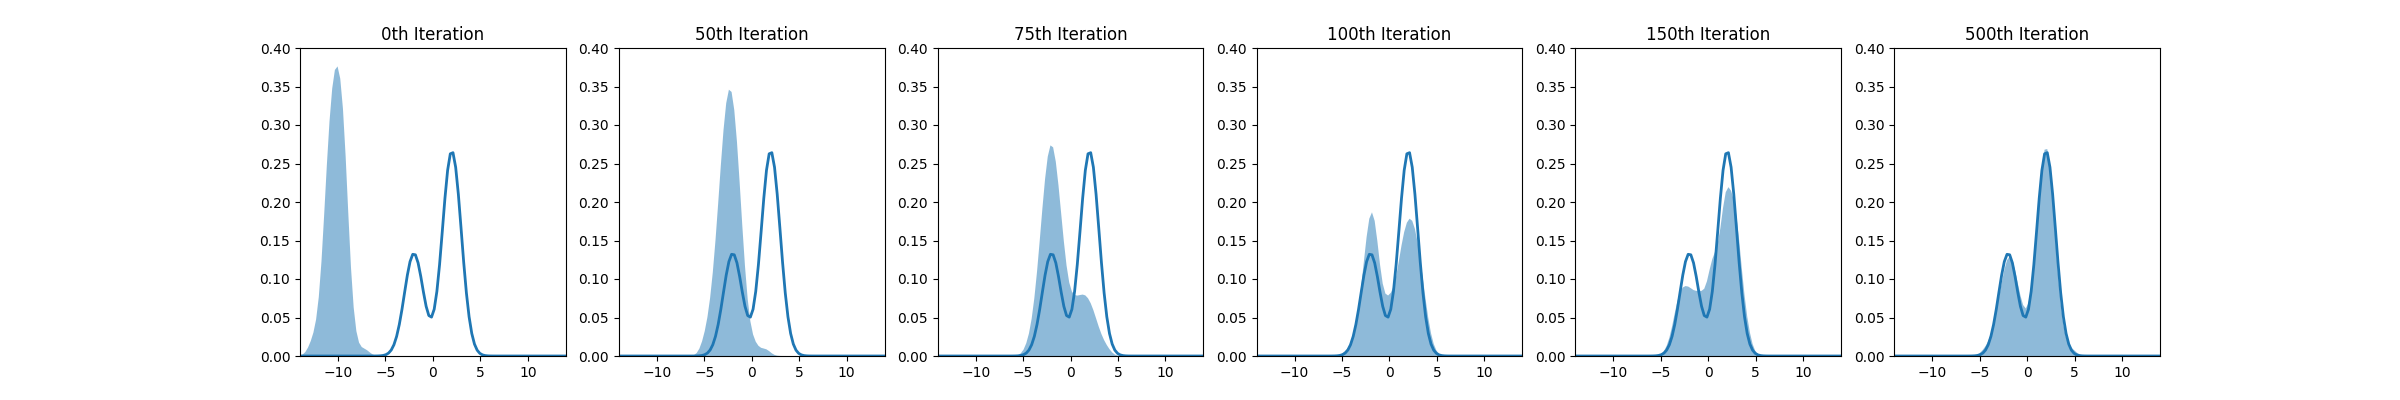
\includegraphics[width=\textwidth]{original-code/Toy-Examples/mixture1d_all.png}
    \caption{Toy example with 1D Gaussian mixture. Particle densities are visualized by KDE.}
    \label{fig:toy1dgaussian-1}
\end{figure}

\begin{figure}[h]
    \centering
    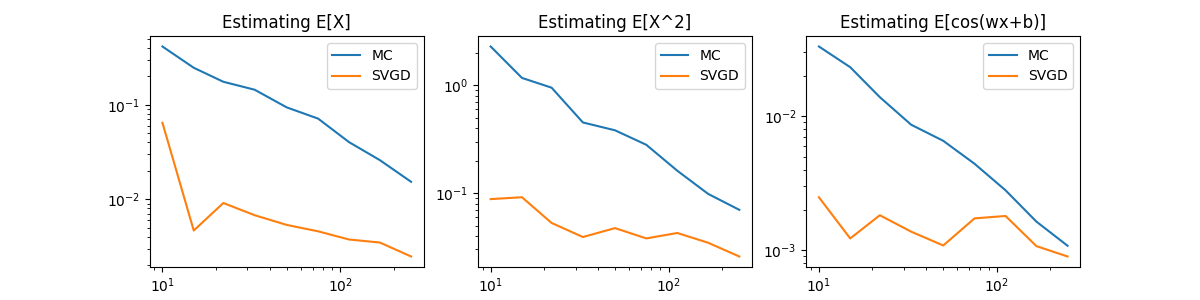
\includegraphics[width=\textwidth]{figs/toy-figure2.png}
    \caption{Comparison between MC and SVGD on simple mean estimation tasks. }
    \label{fig:my_label}
\end{figure}

\subsection{Bayesian Logistic Regression}

We attempt to test the SVGD algorithm in small-scale logistic regression tasks. We aim to construct a model which is able to predict a binary label of some training data. We run the SVGD algorithm as implemented on NumPyro against the No U-Turn Sampler (NUTS) algorithm. We model the logistic regression problem as a model in NumPyro, and simply perform inference on them but using NUTS and SVGD. The result is shown in Figure \ref{fig:logist_small}.



\begin{figure}[h]
    \centering
    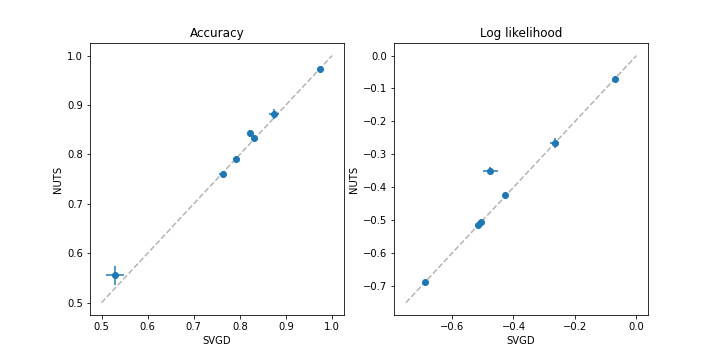
\includegraphics[width=\textwidth]{figs/logistic_svgd_nuts.png}
    \caption{Caption}
    \label{fig:logist_small}
\end{figure}

\subsection{Bayesian Neural Network}

A Bayesian Neural Network (BNN) is a neural network where 

For the experiments, we train a small BNN on a set of regression tasks. We follow the setup from the paper and use the UCI dataset. We run tests on the SVGD algorithm as implemented by the authors of the original paper and also the implementation on NumPyro, and also on the probabilistic back-propagation (PBP) algorithm. A change that we made was to run each algorithms using the same subsaming size of 100 and ran each algorithms for up to 500 epochs. The other hyperparameters were kept the same as the original code. We report the results in Tables \ref{tab:bnn_rmse} and . 

\begin{table}[]
    \centering
\begin{tabular}{|c|ccc|}
\hline
 Dataset & PBP & SVGD (NumPyro) & SVGD (original)  \\
 \hline
boston & $3.039 \pm 0.303$ & $3.430 \pm 0.449$ & $2.999 \pm 0.343$ \\
concrete & $5.699 \pm 0.075$ & $5.661 \pm 0.145$ & $5.763 \pm 0.090$ \\
energy & $1.676 \pm 0.050$ & $1.143 \pm 0.064$ & $1.421 \pm 0.049$ \\
kin8nm & $0.099 \pm 0.001$ & $0.077 \pm 0.001$ & $0.121 \pm 0.001$ \\
naval & $0.006 \pm 0.000$ & $0.001 \pm 0.000$ & $0.008 \pm 0.000$ \\
power & $4.143 \pm 0.050$ & $4.156 \pm 0.051$ & $4.206 \pm 0.049$ \\
protein & $4.680 \pm 0.009$ & $4.518 \pm 0.009$ & $4.859 \pm 0.013$ \\
wine & $0.640 \pm 0.015$ & $0.666 \pm 0.013$ & $0.634 \pm 0.014$ \\
yacht & $0.948 \pm 0.087$ & $1.719 \pm 0.101$ & $1.017 \pm 0.141$ \\
\hline
\end{tabular}
    \caption{Root-mean-squared error (RMSE) on test data for each algorithms} 
    \label{tab:bnn_rmse}
\end{table}

In our results, we were able to replicate the superior performance of the SVGD algorithm over the PBP algorithm.

However, we found that the SVGD algorithm implementation on NumPyro was not able to replicate the performance that the original SVGD algorithm was able to. This could be due to the fact that unlike the SVGD algorithm from the original paper, the SVGD algorithm on NumPyro is minimising the loss based on the ELBO value, and not the true posterior probability. However, to test if this is the 

\begin{figure}[h]
    \centering
    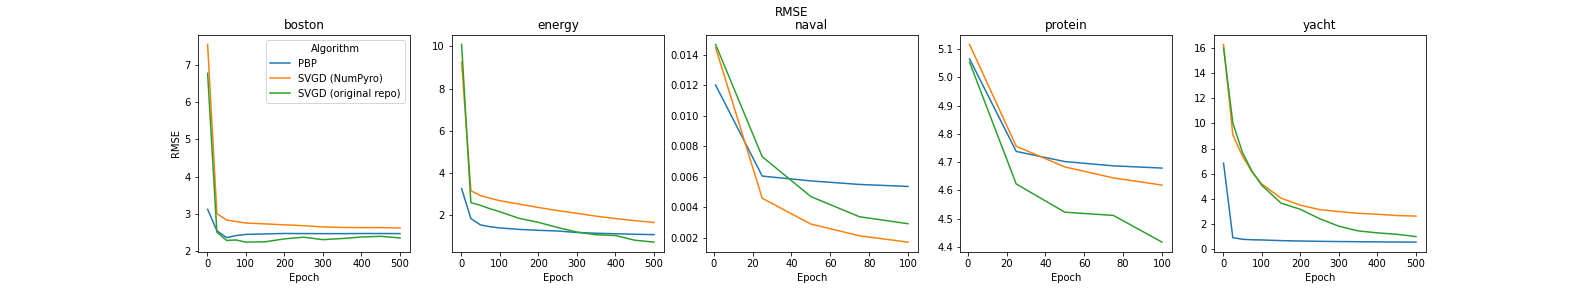
\includegraphics[width=\textwidth]{figs/bayesian_epoch_RMSE.png}
    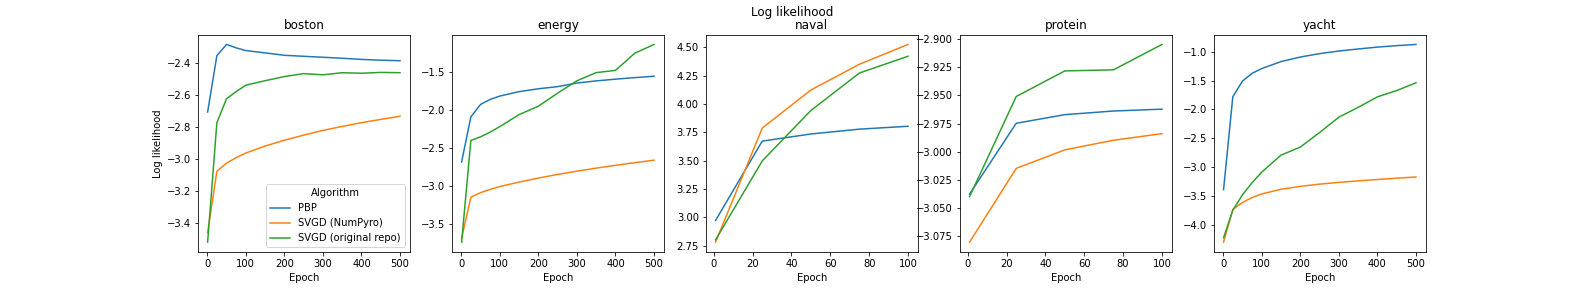
\includegraphics[width=\textwidth]{figs/bayesian_epoch_Loglikelihood.png}
    \caption{Caption}
    \label{fig:my_label}
\end{figure}